%%%%%%%%%%%%%%%%%%%%%%%%%%%%%%%%%%%%%%%%%
% Programming/Coding Assignment
% LaTeX Template
%
% This template has been downloaded from:
% http://www.latextemplates.com
%
% Original author:
% Ted Pavlic (http://www.tedpavlic.com)
%
% Note:
% The \lipsum[#] commands throughout this template generate dummy text
% to fill the template out. These commands should all be removed when 
% writing assignment content.
%
% This template uses a Perl script as an example snippet of code, most other
% languages are also usable. Configure them in the "CODE INCLUSION 
% CONFIGURATION" section.
%
%%%%%%%%%%%%%%%%%%%%%%%%%%%%%%%%%%%%%%%%%

%----------------------------------------------------------------------------------------
%	PACKAGES AND OTHER DOCUMENT CONFIGURATIONS
%----------------------------------------------------------------------------------------

\documentclass{article}

\usepackage{fancyhdr} % Required for custom headers
\usepackage{lastpage} % Required to determine the last page for the footer
\usepackage{extramarks} % Required for headers and footers
\usepackage[usenames,dvipsnames]{color} % Required for custom colors
\usepackage{graphicx} % Required to insert images
\usepackage{subcaption}
\usepackage{listings} % Required for insertion of code
\usepackage{courier} % Required for the courier font
\usepackage{lipsum} % Used for inserting dummy 'Lorem ipsum' text into the template
\usepackage{hyperref} % Used for linking to websites
\usepackage{amsmath, amsthm, amssymb} % Required for writing equations
\usepackage{pythonhighlight} % Required for including Python code

% Margins
\topmargin=-0.45in
\evensidemargin=0in
\oddsidemargin=0in
\textwidth=6.5in
\textheight=9.0in
\headsep=0.25in

\linespread{1.1} % Line spacing

% Set up the header and footer
\pagestyle{fancy}
\lhead{\hmwkAuthorName} % Top left header
\chead{\hmwkClass\ (\hmwkClassTime): \hmwkTitle} % Top center head
%\rhead{\firstxmark} % Top right header
\lfoot{\lastxmark} % Bottom left footer
\cfoot{} % Bottom center footer
\rfoot{Page\ \thepage\ of\ \protect\pageref{LastPage}} % Bottom right footer
\renewcommand\headrulewidth{0.4pt} % Size of the header rule
\renewcommand\footrulewidth{0.4pt} % Size of the footer rule

\setlength\parindent{0pt} % Removes all indentation from paragraphs

%----------------------------------------------------------------------------------------
%	CODE INCLUSION CONFIGURATION
%----------------------------------------------------------------------------------------

\definecolor{MyDarkGreen}{rgb}{0.0,0.4,0.0} % This is the color used for comments
\lstloadlanguages{Perl} % Load Perl syntax for listings, for a list of other languages supported see: ftp://ftp.tex.ac.uk/tex-archive/macros/latex/contrib/listings/listings.pdf
\lstset{language=Perl, % Use Perl in this example
        frame=single, % Single frame around code
        basicstyle=\small\ttfamily, % Use small true type font
        keywordstyle=[1]\color{Blue}\bf, % Perl functions bold and blue
        keywordstyle=[2]\color{Purple}, % Perl function arguments purple
        keywordstyle=[3]\color{Blue}\underbar, % Custom functions underlined and blue
        identifierstyle=, % Nothing special about identifiers                                         
        commentstyle=\usefont{T1}{pcr}{m}{sl}\color{MyDarkGreen}\small, % Comments small dark green courier font
        stringstyle=\color{Purple}, % Strings are purple
        showstringspaces=false, % Don't put marks in string spaces
        tabsize=5, % 5 spaces per tab
        %
        % Put standard Perl functions not included in the default language here
        morekeywords={rand},
        %
        % Put Perl function parameters here
        morekeywords=[2]{on, off, interp},
        %
        % Put user defined functions here
        morekeywords=[3]{test},
       	%
        morecomment=[l][\color{Blue}]{...}, % Line continuation (...) like blue comment
        numbers=left, % Line numbers on left
        firstnumber=1, % Line numbers start with line 1
        numberstyle=\tiny\color{Blue}, % Line numbers are blue and small
        stepnumber=5 % Line numbers go in steps of 5
}

% Creates a new command to include a perl script, the first parameter is the filename of the script (without .pl), the second parameter is the caption
\newcommand{\perlscript}[2]{
\begin{itemize}
\item[]\lstinputlisting[caption=#2,label=#1]{#1.pl}
\end{itemize}
}

%----------------------------------------------------------------------------------------
%	DOCUMENT STRUCTURE COMMANDS
%	Skip this unless you know what you're doing
%----------------------------------------------------------------------------------------

% Header and footer for when a page split occurs within a problem environment
\newcommand{\enterProblemHeader}[1]{
%\nobreak\extramarks{#1}{#1 continued on next page\ldots}\nobreak
%\nobreak\extramarks{#1 (continued)}{#1 continued on next page\ldots}\nobreak
}

% Header and footer for when a page split occurs between problem environments
\newcommand{\exitProblemHeader}[1]{
%\nobreak\extramarks{#1 (continued)}{#1 continued on next page\ldots}\nobreak
%\nobreak\extramarks{#1}{}\nobreak
}

\setcounter{secnumdepth}{0} % Removes default section numbers
\newcounter{homeworkProblemCounter} % Creates a counter to keep track of the number of problems
\setcounter{homeworkProblemCounter}{0}

\newcommand{\homeworkProblemName}{}
\newenvironment{homeworkProblem}[1][Part \arabic{homeworkProblemCounter}]{ % Makes a new environment called homeworkProblem which takes 1 argument (custom name) but the default is "Problem #"
\stepcounter{homeworkProblemCounter} % Increase counter for number of problems
\renewcommand{\homeworkProblemName}{#1} % Assign \homeworkProblemName the name of the problem
\section{\homeworkProblemName} % Make a section in the document with the custom problem count
\enterProblemHeader{\homeworkProblemName} % Header and footer within the environment
}{
\exitProblemHeader{\homeworkProblemName} % Header and footer after the environment
}

\newcommand{\problemAnswer}[1]{ % Defines the problem answer command with the content as the only argument
\noindent\framebox[\columnwidth][c]{\begin{minipage}{0.98\columnwidth}#1\end{minipage}} % Makes the box around the problem answer and puts the content inside
}

\newcommand{\homeworkSectionName}{}
\newenvironment{homeworkSection}[1]{ % New environment for sections within homework problems, takes 1 argument - the name of the section
\renewcommand{\homeworkSectionName}{#1} % Assign \homeworkSectionName to the name of the section from the environment argument
\subsection{\homeworkSectionName} % Make a subsection with the custom name of the subsection
\enterProblemHeader{\homeworkProblemName\ [\homeworkSectionName]} % Header and footer within the environment
}{
\enterProblemHeader{\homeworkProblemName} % Header and footer after the environment
}

%----------------------------------------------------------------------------------------
%	NAME AND CLASS SECTION
%----------------------------------------------------------------------------------------

\newcommand{\hmwkTitle}{Assignment\ \#1} % Assignment title
\newcommand{\hmwkDueDate}{Monday,\ January\ 29,\ 2018} % Due date
\newcommand{\hmwkClass}{CSC411} % Course/class
\newcommand{\hmwkClassTime}{L2501} % Class/lecture time
\newcommand{\hmwkAuthorName}{Chawla Dhruv} % Your name

%----------------------------------------------------------------------------------------
%	TITLE PAGE
%----------------------------------------------------------------------------------------

\title{
\vspace{2in}
\textmd{\textbf{\hmwkClass:\ \hmwkTitle}}\\
\normalsize\vspace{0.1in}\small{Due\ on\ \hmwkDueDate}\\
\vspace{0.1in}
\vspace{3in}
}

\author{\textbf{\hmwkAuthorName}}
%\date{} % Insert date here if you want it to appear below your name

%----------------------------------------------------------------------------------------

\begin{document}

\maketitle
\clearpage

%----------------------------------------------------------------------------------------
%	PART 1
%----------------------------------------------------------------------------------------

\begin{homeworkProblem}

\noindent \textit{Dataset description}\\

The dataset (in the \texttt{cropped} folder) is a collection of 32x32 grayscale images, which are cropped and converted from a subset of FaceScrub dataset provided on the \href{http://www.teach.cs.toronto.edu/~csc411h/winter/projects/proj1/}{CSC411 Project1 webpage}.\\

The images are primarily headshots which display the actor's forehead, eyes (in some cases the actors are wearing transparent glasses), nose, mouth (can be closed, or donning a smile or a laugh) and chin.\\

Most of the images are shot straight on (with some exceptions where the head is turned slightly to the side) and in adequate lighting having minimal shadows on the actors' faces.\\

The images are labeled as \texttt{<actor\_name>\_<i>.jpg} where \texttt{i} is a number greater than 0 (like a counter) and \texttt{actor\_name} is last name of an actor in lower case.\\

Some random examples from the images (cropped and uncropped) are shown \\

\begin{figure*}[h!]
	\centering 
	\begin{subfigure}{0.35\textwidth}
		\centering
		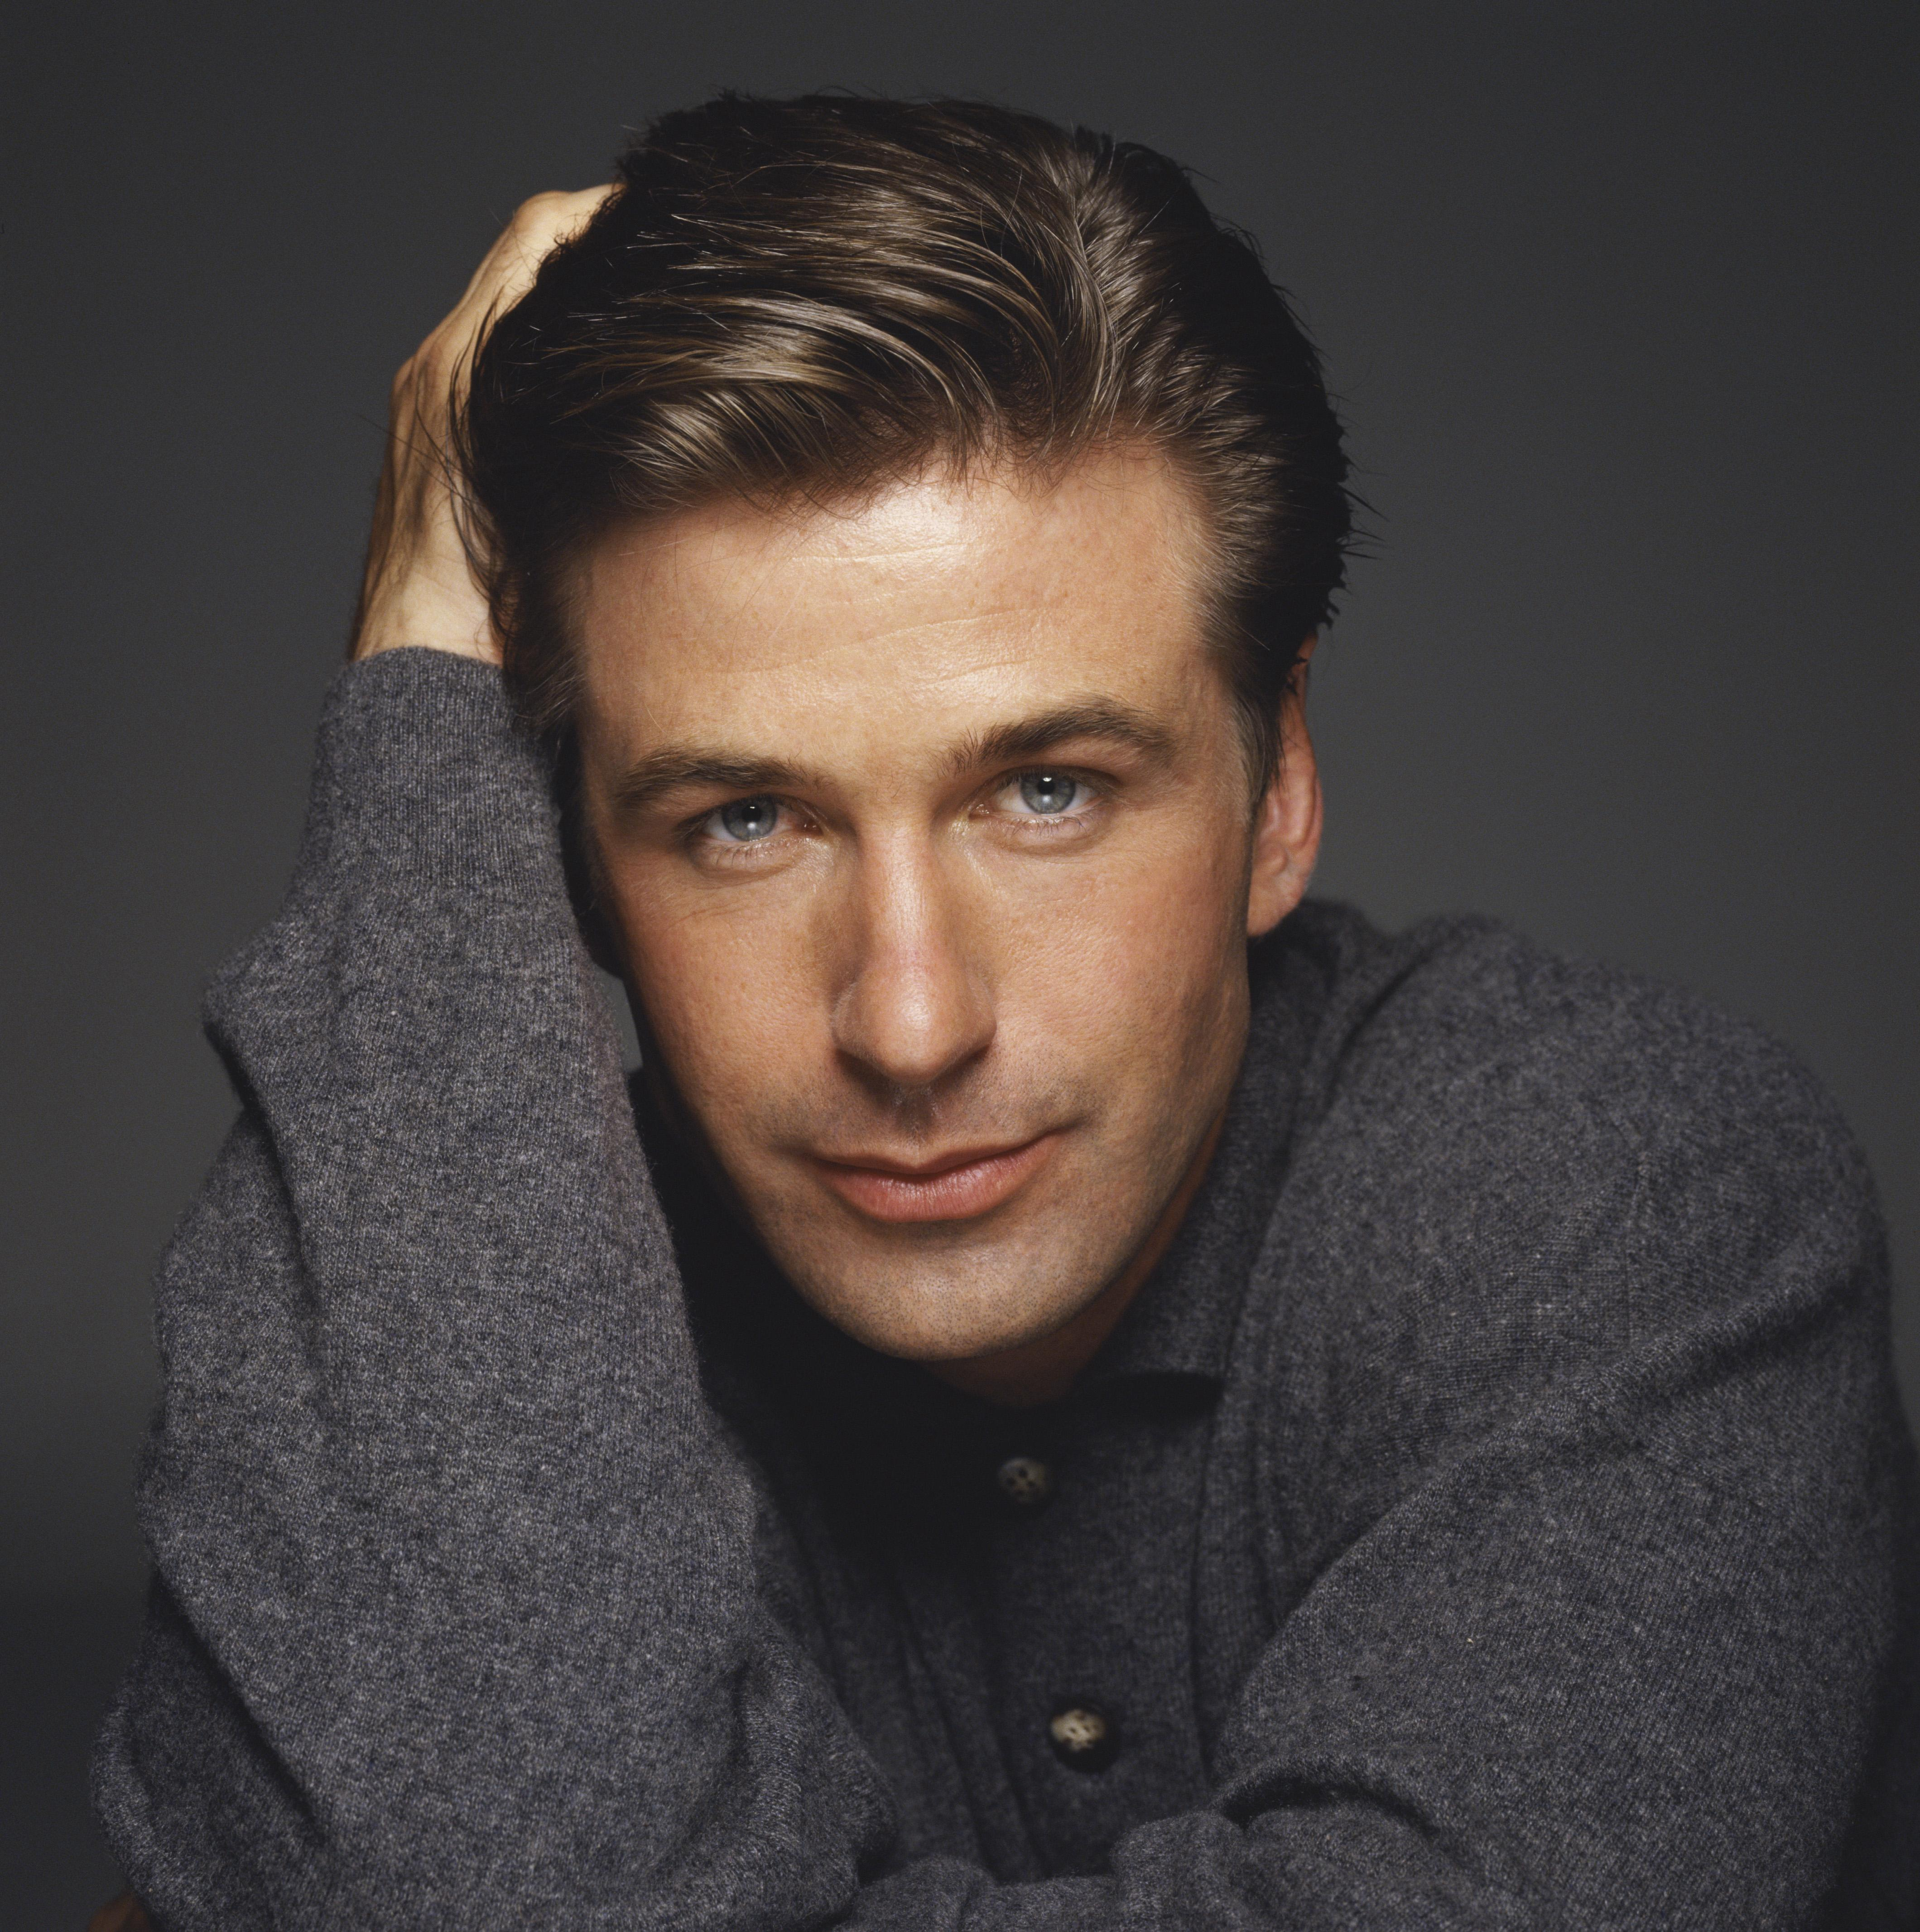
\includegraphics[scale=0.03]{part1_uncropped1.jpg}
		\caption{Alec Baldwin Uncropped}
		\label{fig:sfig1}
	\end{subfigure}
	\begin{subfigure}{0.35\textwidth}
		\centering
		
\includegraphics[scale=1]{part1_cropped1.jpg}
		\caption{Alec Baldwin Cropped}
		\label{fig:sfig2}
	\end{subfigure}
	\begin{subfigure}{0.35\textwidth}
		\centering
		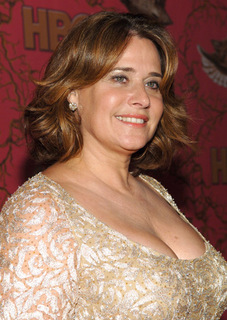
\includegraphics[scale=0.3]{part1_uncropped2.jpg}
		\caption{Lorraine Bracco Uncropped}
		\label{fig:sfig3}
	\end{subfigure}
	\begin{subfigure}{0.35\textwidth}
		\centering
		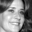
\includegraphics[scale=1]{part1_cropped2.jpg}
		\caption{Lorraine Bracco Cropped}
		\label{fig:sfig4}
	\end{subfigure}
	\begin{subfigure}{0.35\textwidth}
		\centering
		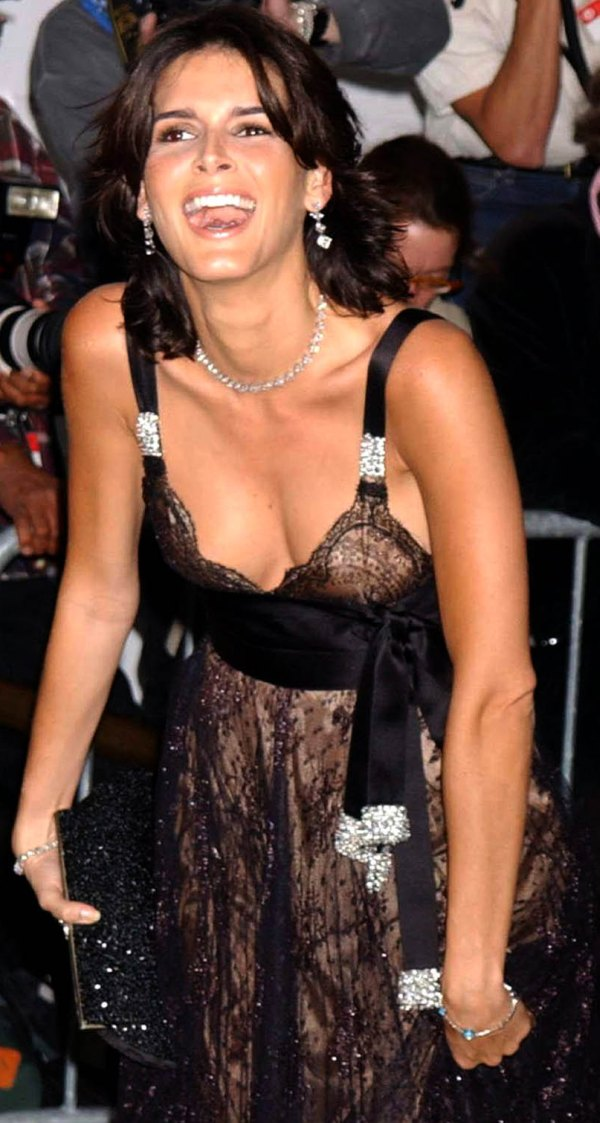
\includegraphics[scale=0.3]{part1_uncropped3.jpg}
		\caption{Angie Harmon Uncropped}
		\label{fig:sfig5}
	\end{subfigure}
	\begin{subfigure}{0.35\textwidth}
		\centering
		
\includegraphics[scale=1]{part1_cropped3.jpg}
		\caption{Angie Harmon Cropped}
		\label{fig:sfig6}
	\end{subfigure}
	\caption{Examples of uncropped images of 3 actors in the dataset along with their cropped images}
	\label{fig:fig1}
\end{figure*}

\clearpage

\noindent \textit{Procedure for constructing the dataset}

The two datasets from \href{http://www.teach.cs.toronto.edu/~csc411h/winter/projects/proj1/}{CSC411 Project1 webpage} are combined into one single text file, \texttt{faces\_subset.txt}. The \texttt{get\_and\_crop\_images} function, which takes in a list of actors, finds the links for actors in \texttt{faces\_subset.txt}, downloads the raw image, crops them into 32x32 using bounding boxes specified in \texttt{faces\_subset.txt}, and saves them as grayscale.\\

A second function \texttt{remove\_bad\_images} can then be called to remove images with incorrect bounding boxes or poor image quality (such as blur or dark shadows) from \texttt{cropped} folder. \texttt{remove\_bad\_images} has a list manually chosen that removes bad images for datasets for all 12 actors in \texttt{faces\_subset.txt}\\

\noindent \textit{Tip: Unzip cropped.zip to get all dataset images without having to bother downloading them all yourself.}

\end{homeworkProblem}
\clearpage

%----------------------------------------------------------------------------------------
%	PART 2
%----------------------------------------------------------------------------------------

\begin{homeworkProblem}

\noindent \textit{Splitting the dataset into training, validation and testing sets}\\

The function \texttt{build\_sets} takes in the name of an actor (example: \textit{gilpin}) and returns three lists, \texttt{training\_set}, \texttt{validation\_set} and \texttt{testing\_set}. \texttt{validation\_set} and \texttt{testing\_set} are both 10 images each while \texttt{training\_set} is the remainder from the rest of the actor's dataset.\\

\textit{Note: All three lists are \textbf{non-overlapping}}\\

The lists are made using \texttt{numpy.random.shuffle()}. A seed of 5 is chosen to ensure reproducibility.\\

Here's an example of \texttt{build\_sets} in action.

\begin{verbatim}
>>> training_set, validation_set, testing_set = build_sets('bracco')
>>> training_set
['bracco58.jpg', 'bracco55.jpg', 'bracco102.jpg', 'bracco109.jpg', 'bracco13.jpg',
 'bracco118.jpg', 'bracco78.jpg', 'bracco8.jpg', 'bracco31.jpg', 'bracco36.jpg', 
 'bracco49.jpg', 'bracco119.jpg', 'bracco17.jpg', 'bracco63.jpg', 'bracco71.jpg', 
 'bracco44.jpg', 'bracco73.jpg', 'bracco106.jpg', 'bracco96.jpg', 'bracco42.jpg', 
 'bracco32.jpg', 'bracco68.jpg', 'bracco84.jpg', 'bracco113.jpg', 'bracco57.jpg', 
 'bracco6.jpg', 'bracco27.jpg', 'bracco116.png', 'bracco41.JPG', 'bracco56.jpg', 
 'bracco91.jpg', 'bracco33.jpg', 'bracco45.jpg', 'bracco83.jpg', 'bracco117.jpg', 
 'bracco52.jpg', 'bracco47.jpg', 'bracco28.jpg', 'bracco103.jpg', 'bracco43.jpg', 
 'bracco48.jpg', 'bracco60.jpg', 'bracco2.jpg', 'bracco54.jpg', 'bracco66.jpg', 
 'bracco82.jpg', 'bracco74.jpg', 'bracco4.jpg', 'bracco76.jpg', 'bracco21.jpg', 
 'bracco98.jpg', 'bracco112.jpg', 'bracco114.jpg', 'bracco53.jpg', 'bracco19.jpg', 
 'bracco16.jpg', 'bracco9.jpg', 'bracco104.jpg', 'bracco30.jpg', 'bracco100.jpg', 
 'bracco87.jpg', 'bracco69.jpg', 'bracco40.jpg', 'bracco10.jpg', 'bracco7.jpg', 
 'bracco38.jpg', 'bracco12.jpg', 'bracco97.jpg', 'bracco108.jpg', 'bracco95.jpg', 
 'bracco92.jpg', 'bracco81.jpg', 'bracco26.jpg', 'bracco46.jpg', 'bracco18.jpg', 
 'bracco120.jpg', 'bracco23.jpg', 'bracco80.jpg', 'bracco61.jpg', 'bracco62.jpg', 
 'bracco107.jpg', 'bracco70.jpg', 'bracco105.jpg', 'bracco20.jpeg', 'bracco22.jpg', 
 'bracco101.jpg', 'bracco35.jpg', 'bracco86.jpg', 'bracco34.jpg', 'bracco85.jpg', 
 'bracco29.jpg', 'bracco14.jpg', 'bracco115.jpg', 'bracco88.jpg', 'bracco67.jpg', 
 'bracco24.jpg', 'bracco37.jpg']
>>> validation_set
['bracco3.jpg', 'bracco99.jpg', 'bracco111.jpg', 'bracco122.jpg', 'bracco25.jpg', 
'bracco75.jpg', 'bracco94.jpg', 'bracco65.jpg', 'bracco39.jpg', 'bracco5.jpg']
>>> testing_set
['bracco0.jpg', 'bracco93.jpg', 'bracco15.jpg', 'bracco89.jpg', 'bracco79.jpg', 
'bracco59.jpg', 'bracco72.jpg', 'bracco11.jpg', 'bracco1.jpg', 'bracco51.jpg']
\end{verbatim}

\end{homeworkProblem}
\clearpage

%----------------------------------------------------------------------------------------
%	PART 3
%----------------------------------------------------------------------------------------

\begin{homeworkProblem}

\noindent \textit{Binary Classfier: Steve Carell or Alec Baldwin?}\\

\textbf{Cost function minimized: }Squared Error\\\\
\textbf{Cost function value for training set: }4.12004741282\\
\textbf{Cost function value for validation set: }1.53816055196\\\\
\textbf{Performance on training set: }100\% (on more than 200 images with a near equal distribution of Steve Carell and Alec Baldwin images)\\
\textbf{Performance on validation set: }95\% (on 20 images: 10 of Steve Carell and 10 of Alec Baldwin)\\\\
\textbf{Alpha: }$10^{-5}$ \\
\textbf{Number of iterations: }5000\\\\

Here's my code for computing the output of the classifier (from \texttt{part3()} of \texttt{faces.py})\\

\begin{python}
correct, total, cost_fn = 0, 0, 0

for v_0 in validation_set_0:
    v_img = imread("cropped/"+v_0)
    v_img = rgb2gray(v_img)
    v_img = reshape(np.ndarray.flatten(v_img), [1, 1024])
    v_img = np.insert(v_img, 0, 1)

    prediction = dot(theta.T, v_img)

    cost_fn += (1 - prediction)**2

    if linalg.norm(prediction) > 0.5: correct += 1
    total += 1

for v_1 in validation_set_1:
    v_img = imread("cropped/"+v_1)
    v_img = rgb2gray(v_img)
    v_img = reshape(np.ndarray.flatten(v_img), [1, 1024])
    v_img = np.insert(v_img, 0, 1)

    prediction = dot(theta.T, v_img)

    cost_fn += (prediction)**2

    if linalg.norm(prediction) < 0.5: correct += 1
    total += 1

print("Validation Set Performance = "+str(correct)+"/"+str(total))
print("Cost Function value for validation set is "+str(cost_fn))
\end{python}

\texttt{validation\_set\_0} and \texttt{validation\_set\_1} are validation sets for Alec Baldwin and Steve Carell respectively.\\

A similar piece of code measures classifier performance on training sets.\\

\clearpage

\textit{Procedure to fine-tune system performance}\\

First I started of with 50,000 iterations and $\alpha = 10^{-7}$. I increased the number of iterations until I observed the cost function for validation sets increasing. I increased $\alpha$ to $10^{-6}$ and reduced iterations to bring down the validation set cost. I continued this process of increasing $\alpha$ and reducing iterations until the cost function of training set started to increase and performance started going down. This is where I stopped my process and got my presented classifier performance and cost values.\\

If $\alpha$ was made too large, the python compiler would throw an overflow error in the calculation of the dot product between $\theta$ transpose and $\alpha$.\\

\end{homeworkProblem}
\clearpage

%----------------------------------------------------------------------------------------
%	PART 4
%----------------------------------------------------------------------------------------

\begin{homeworkProblem}

\noindent \textit{Displaying thetas}\\

\begin{figure*}[h!]
	\centering 
	\begin{subfigure}{0.45\textwidth}
		\centering
		
\includegraphics[scale=2]{part4a_1.jpg}
		\\4(a): Full training set
	\end{subfigure}
	\begin{subfigure}{0.45\textwidth}
		\centering
		
\includegraphics[scale=2]{part4a_2.jpg}
		\\4(a): Reduced training set with 2 images of each actor
	\end{subfigure}
	\begin{subfigure}{0.45\textwidth}
		\centering
		
\includegraphics[scale=2]{part4b_1.jpg}
		\\4(b): Gradient descent run with 5,000 iterations
	\end{subfigure}
	\begin{subfigure}{0.45\textwidth}
		\centering
		
\includegraphics[scale=2]{part4b_2.jpg}
		\\4(b): Gradient descent run with only 10 iterations
	\end{subfigure}
	\caption{Displaying $\theta$ using combination of full or reduced training set and number of iterations}
	\label{fig:fig2}
\end{figure*}

As can be seen, training with less iterations and with less training examples results in the $\theta$s resembling actual human faces more. This can be explained as training with more iterations and more training examples goes into the territory of overfitting and spurious details start showing up and we lose regular features.\\

\end{homeworkProblem}
\clearpage

%----------------------------------------------------------------------------------------
%	PART 5
%----------------------------------------------------------------------------------------

\begin{homeworkProblem}

\noindent \textit{Gender Classification: Overfitting}\\

\begin{figure*}[h!]
	\centering
	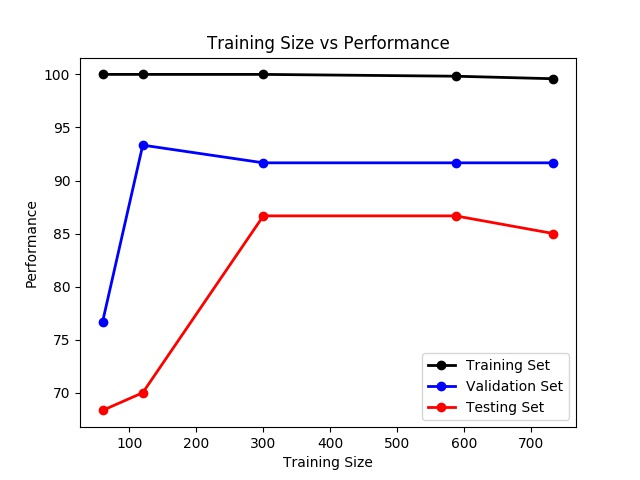
\includegraphics[scale=0.75]{part5.jpg}
	\caption{Performance (in \%) on training, validation and test sets as size of training set increases}
	\label{fig:fig3}
\end{figure*}

\noindent \textit{Parameters}\\

\textbf{Alpha: }$10^{-6}$\\
\textbf{Iterations: }$80,000$\\\\

The performance on the training set stays at around 100\% while validation set performance reaches its maximum at around 120 training images and then drops by 2\% while the performance on test set starts dropping after 600 training images.\\

The reduction in performance for the testing and validation set as the number of training examples increase clearly demonstrates overfitting.\\

\end{homeworkProblem}
\clearpage

%----------------------------------------------------------------------------------------
%	PART 6
%----------------------------------------------------------------------------------------

\begin{homeworkProblem}

\noindent \textit{Multi Classifiication}\\

%	PART A
\subsection{Part A}
\begin{gather*}
J(\theta) = \sum_{i} (\sum_{j} (\theta^{T} x^{(i)} - y^{(i)})^2_j)
\end{gather*}
\begin{equation}
\begin{split}
\frac {\partial J} {\partial \theta_{pq}} & = \sum_{i} \frac {\partial } {\partial \theta_{pq}} (\theta^{(i)}_0 x^{(i)}_0 + ... + \theta^{(i)}_q x^{(i)}_q + ... + \theta^{(i)}_k x^{(i)}_k - y^{(i)}_0 - ... - y^{(i)}_q - ... - y^{(i)}_k)^2\\
& = \frac {\partial } {\partial \theta_{pq}} (\theta^{(p)}_0 x^{(p)}_0 + ... + \theta^{(p)}_q x^{(p)}_q + ... + \theta^{(p)}_k x^{(p)}_k - y^{(p)}_0 - ... - y^{(p)}_q - ... - y^{(p)}_k)^2\\
&=  2 x^{(p)}_q (\theta^{(p)}_q x^{(p)}_q - y^{(p)}_q)\\
\end{split}
\end{equation}

%	PART B
\subsection{Part B}
\begin{gather}
\frac {\partial J} {\partial \theta} = 
\begin{bmatrix}
	\frac {\partial J} {\partial \theta_{11}} & \frac {\partial J} {\partial \theta_{12}} & \dots & \frac {\partial J} {\partial \theta_{1k}}\\
	\vdots & \vdots & \ddots & \vdots\\
	\frac {\partial J} {\partial \theta_{n1}} & \frac {\partial J} {\partial \theta_{n2}} & \dots & \frac {\partial J} {\partial \theta_{nk}}
\end{bmatrix}\\
\frac {\partial J} {\partial \theta} = 
\begin{bmatrix}
	2 x_1 (\theta^{T} x - y)_1 & 2 x_1 (\theta^{T} x - y)_2 & \dots & 2 x_1 (\theta^{T} x - y)_k\\
	\vdots & \vdots & \ddots & \vdots\\
	2 x_n (\theta^{T} x - y)_1 & 2 x_n (\theta^{T} x - y)_2 & \dots & 2 x_n (\theta^{T} x - y)_k\\
\end{bmatrix}\\
\frac {\partial J} {\partial \theta} = 2 
\begin{bmatrix}
	x_1\\ x_2\\ \vdots \\ x_n
\end{bmatrix}
\begin{bmatrix}
	(\theta^{T} x - y)_1 & (\theta^{T} x - y)_2 & \hdotsfor{1} & (\theta^{T} x - y)_k
\end{bmatrix}\\
\frac {\partial J} {\partial \theta} = 2 X (\theta^{T} X - Y)^{T}
\end{gather}

%	PART C
\subsection{Part C}

The cost function from 6(a) is as below:\\
\begin{python}
def f_multiclass(x, y, theta):
    x = np.transpose(x)
    x = vstack((ones((1, x.shape[1])), x))
    return sum( (y - dot(x.T, theta.T)) ** 2)
\end{python}

The code for vectorized gradient function is:
\begin{python}
def df_multiclass(x, y, theta):
    x = np.transpose(x)
    x = vstack( (ones((1, x.shape[1])), x))
    return 2*(dot(x, (dot(theta, x)).T-y)).T

def grad_descent_multiclass(f, df, x, y, init_t, alpha, max_iter = 20000):
    EPS = 1e-10   
    prev_t = init_t-10*EPS
    t = init_t.copy()
    ite  = 0

    while norm(t - prev_t) >  EPS and ite < max_iter:
        prev_t = t.copy()
        t -= alpha*df(x, y, t)
        if ite % 5000 == 0 or ite == max_iter-1:
            print "Iter", ite
            print "Gradient: ", df(x, y, t), "\n"
        ite += 1
    return t
\end{python}

\textit{The above functions are present in} \texttt{calculus.py}

%	PART D
\subsection{Part D}

\end{homeworkProblem}
\clearpage

%----------------------------------------------------------------------------------------
%	PART 7
%----------------------------------------------------------------------------------------

\begin{homeworkProblem}

\noindent \textit{Multi face recognition}\\

\textbf{Performance on training set: }94\%\\
\textbf{Performance on validation set: }71.67\%\\\\
\textbf{Alpha: }$10^{-7}$ \\
\textbf{Number of iterations: }150,000\\\\

A small value of $\alpha$ was chosen to obtain more accurate classifier performance and number of iterations were chosen to the same effect while trying to avoid overfitting the model.\\

\noindent \textit{Obtaining label from output of model}\\

To obtain label from the output of the model, we find the index of maximum element in \texttt{numpy.dot(theta, x)} and find the label that correspronds to that index in the training set.\\

For example, if \texttt{numpy.dot(theta, x)} comes out to be \texttt{[0.1, 0.2, 0.38, 0.83, 0.56, 0.17]}, the 3\textsuperscript{rd} index has the highest element which corresponds to Alec Baldwin.

\end{homeworkProblem}
\clearpage

%----------------------------------------------------------------------------------------
%	PART 8
%----------------------------------------------------------------------------------------

\begin{homeworkProblem}

\noindent \textit{Visualising thetas for different actors}\\

\begin{figure*}[h!]
	\centering 
	\begin{subfigure}{0.35\textwidth}
		\centering
		
\includegraphics[scale=4]{part8_0.jpg}
		\caption{Lorraine Bracco}
		\label{fig:sfig1}
	\end{subfigure}
	\begin{subfigure}{0.35\textwidth}
		\centering
		
\includegraphics[scale=4]{part8_1.jpg}
		\caption{Peri Gilpin}
		\label{fig:sfig2}
	\end{subfigure}
	\begin{subfigure}{0.35\textwidth}
		\centering
		
\includegraphics[scale=4]{part8_2.jpg}
		\caption{Angie Harmon}
		\label{fig:sfig3}
	\end{subfigure}
	\begin{subfigure}{0.35\textwidth}
		\centering
		
\includegraphics[scale=4]{part8_3.jpg}
		\caption{Alec Baldwin}
		\label{fig:sfig4}
	\end{subfigure}
	\begin{subfigure}{0.35\textwidth}
		\centering
		
\includegraphics[scale=4]{part8_4.jpg}
		\caption{Bill Hader}
		\label{fig:sfig5}
	\end{subfigure}
	\begin{subfigure}{0.35\textwidth}
		\centering
		
\includegraphics[scale=4]{part8_5.jpg}
		\caption{Steve Carell}
		\label{fig:sfig6}
	\end{subfigure}
	\caption{Visualising $\theta$s for different actors in the training set}
	\label{fig:fig4}
\end{figure*}

\end{homeworkProblem}
\clearpage

%----------------------------------------------------------------------------------------

\end{document}